\par Durant notre stage de fin d’études, nous avons eu la chance de travailler au sein d’une équipe opérationnelle et bien organisée, dont les membres sont dotés de l’esprit d’équipe, d’entre-aide et du sens d’initiative et de créativité.
\par Dans la présente Section, on va découvrir ces équipes là et les projets aux quel j'ai eu la chance de contribuer.

\begingroup
\let\clearpage\relax
\chapter{OST/ITS/INV/MDM}
\endgroup

\par Comme toutes les grandes multinationales, Amundi AM recense un nombre incalculable de départements, de secteurs ou d'équipes. Dans le chapitre suivant, je vais décrire l’organisation générale des deux équipes où j’ai effectué mon stage, en suivant une approche descendante.
\\~\\

\section{OST: Operations Services \& Technologies}

\par Amundi AM est subdivisée en plusieurs entités principales (nommée Divisions), on retrouve notamment les départements administrant le groupe Amundi AM (par exemple le département DGL, présidé par Mr. Perrier Yves, président et directeur général du groupe Amundi), les départements relatifs au relations clients Amundi AM (par exemple INS: Institutional Clients Division, RET: Retail Clients Division \dots). Ensuite on retrouve les divisions responsables des activités d'Amundi AM, a savoir BSC (Business Support \& Control) et OST (Operations services \& Technologies). 
\par Présidé par Mr. Lesage Guillaume, cette division regroupe les différents départements essentiels a la gestions d'actifs, activité principale d'Amundi AM. On retrouve par exemple le service NEG (Negociation), ASM (Asset Servicing Management), ASV (Amundi Services) et AFN (Amundi Finance). En plus de ces départements, la division contient aussi ITS (Amundi Technology, IT Services), département auquel j'ai été affecté, qui contient à son tour plusieurs services. 
\clearpage
\section{ITS: Amundi Technology, IT Services}

\begin{figure}[ht]
    \centering
    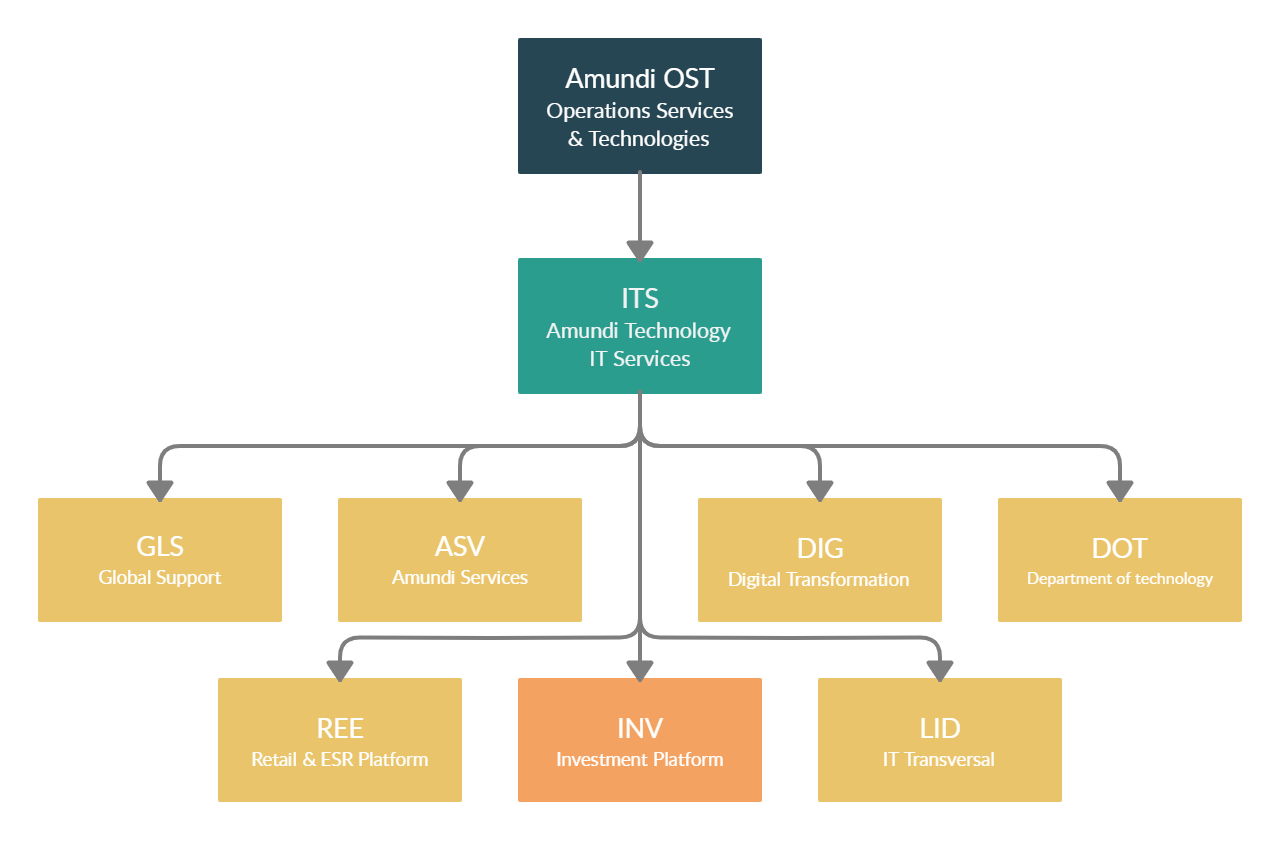
\includegraphics[width=\columnwidth]{img/Org ITS.png}
    \caption{Organisation ITS}
    \label{fig:its}
\end{figure}

\par Le département ITS, comme le nom l'indique, est le département responsable de tout ce qui est service IT. Il est composé de sept services comme le montre la figure \ref{fig:its} ci-dessus: 
\begin{itemize}
    \item GLS (Global Support): la branche d'Amundi ITS basé à Dublin (Irlande) subdivisée en deux services, DHB (Dublin Hub and Intl. Development)\& DOT (Department of technology: Dublin Hub and infrastructure)
    \item ASV (Amundi Services): Amundi services (cf. Part I. Chapitre II.)
    \item DIG (Digital Transformation): Service mutualisé avec le département BSC (Business support and control) chargé de la transformation et communication digitale.
    \item DOT (Department of technology): regroupe les équipes qui travaillent sur le côté hardware (architecture, infrastructure et réseaux), Frameworks internes (dont un que j'ai eu la chance d'utiliser dans un projet) et gestion de base de données. 
    \item REE (Retail \& ESR Platform): Service gérant deux applications Amundi AM majeurs, Alto Retail et ESR. 
    \item LID (IT Transversal): Leading IT Department
    \item INV (Investment Management Platform): Service qui est subdivisé en plusieurs équipes, responsables de plusieurs applications client et interne Amundi AM. Service auquel j'ai été affecté et qu'on va détailler dans la prochaine section
\end{itemize}

\section{INV: Investment Management Platform}
\par Comme c'est déjà mentionné dans la précédente section, le service INV est subdivisé en plusieurs équipes (comme le montre la figure \ref{fig:inv} ci-dessous).\\
\begin{itemize}
    \item EAX: Entreprise Architecture \& UX Design, Equipe qui ce charge de tout ce qui design et maquettes d'applications (User Interface, User Experience) (Notamment utilisé dans le projet Alto Investment Research cf. XXXX) 
    \item FOA: Front Office \& Analysis, Equipe qui se charge des projets Front office (cf. Partie I. Chapitre II. Section I. Sous-Section "Organisation d'un Asset Manager")
    \item RIS: Risk Development
    \item DHB: Dublin Hub Development, précédemment cité dans la Section 2 du Chapitre I. de la partie II. est l'equipe INV basée a Dublin (Irlande). Elle se compose principalement du projet PKC (Position Keeping \& Control) 
    \item INS: Institutional 
    \item TTP: Trading \& MO Trade Processing 
    \item MDM: Master Data Management, Equipe a laquelle je suis affecté, la prochaine section de ce chapitre essayera de détailler ses missions, applications gérés, et périmètre de fonctions.
\end{itemize}
\par Chaque équipe gère des applications essentiels au activités d'Amundi AM.
\begin{figure}[ht]
    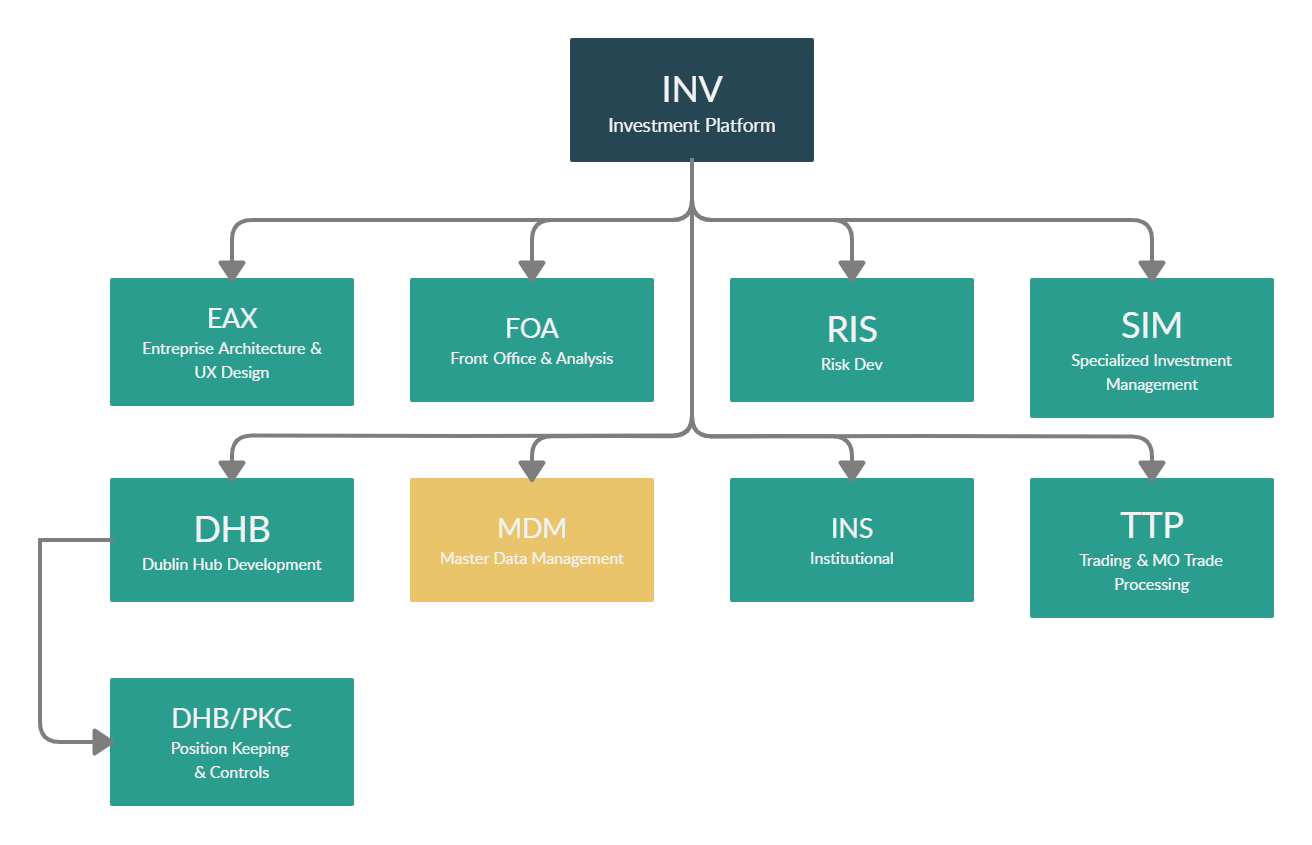
\includegraphics[width=\columnwidth]{img/Org INV.png}
    \caption{Organisation INV}
    \label{fig:inv}
\end{figure}

\section{MDM: Master Data management}
\par MDM, ou Master Data Management, est le département responsable de toutes les application gérant les données utilisé par le métier Amundi (Exemple: portefeuilles, positions, données marchés\dots)(communément appelé Master Data).
\par On dénombre pour le moment sept projets majeurs:
\begin{itemize}
    \item Life : C'est le projet d'implémentation de DataHub, au sein d'Amundi, en vue d'une gestion des référentiels tiers en valeurs et indices. Ce projet a aussi pour but de traiter l’obsolescence ainsi que l'optimisation d’une partie du SI Référentiels.
    \item Medco: ou MediaPlus-core est l'un des projets les plus importants de MDM. C'est le serveur de diffusion, en date du jour, de données principale, notamment pour les portefeuilles et instruments (et tout donnée relatifs). Le but étant de Sérialiser et cacher (transformer en Caches) des objets qui sont des mappings JAVA d'une ou plusieurs tables de base de données. Ceci permet d'avoir un accès direct a ces donnes via l'API MediaPlus-core pour tout client du serveur.
    \item Refgt: ou Referential Gate est un autre serveur de diffusion, mais pour le coup, en date passée. Le serveur récupère ses données depuis plusieurs sources notamment Medco ainsi que des différentes tables de bases de données, pour les historiser. Le serveur permet aussi d'écrire certain types de data dans les différentes tables de bases de données. 
    \item Hubref: ou Refrential Hub, est un serveur de routage, il permet selon le besoin de récupérer la data depuis RefGate ou Medco et de la diffuser a son tour. Ce serveur est notamment utilisé par plusieurs applications front comme Alto Investment Research.
    \item Atlas: Cet application Master Data Management se charge de collecter, intégrer, administrer et diffuser la data qui provient des partenaires d'Amundi AM.
    \item Indice: est une application/serveur qui gère tout autour de deux types d'instruments financier, les indices et benchmarks. 
    \item Alto Investment Research - Refrential Widgets : Alto (Amundi Leading Technologies and Operations) Investment Research est une application subdivisée entre 3 équipes, une partie pour l'équipe appartenant à ITS/DOT/COR (équipe qui se charge du développement du Framework Maestro, Framework sur lequel est basé l'application), une partie pour l'équipe appartenant à ITS/INV/FOA (équipe en charge de différents types de Data) et la partie assignée à l'équipe ITS/INV/MDM, la partie sur la quelle on gère la data reçu par Hubref.
\end{itemize}

\par En plus de ces sept projets on dénombre plusieurs plus petit projets, ou des projets dont le périmètre de fonctions est plutôt éloigné du contexte de mon stage de fin d'études, on peut notamment citer : MDBM, MDQC, FundLife, DQC, Libra \dots   
\par De mon coté, j'ai été assigné au projet MediaPlus-Core puis au projet Alto Investment Research sur la partie Referential Widgets.
\par Le chapitre suivant apportera plus d'informations sur les deux projets, ainsi que des schémas expliquant le fonctionnement et l'environnement technique de chaque projet.


\chapter{Projets}
\par Durant le présent chapitre, on essayera de projeter plus d'informations sur les deux projets auquel j'ai eu la chance d'être affecté, à savoir MediaPlus-core et Alto Investment Research. On présentera chaque projet, son utilité, ses fonctions, son architecture ainsi que son environnement technique.
\section{MediaPlus-Core}
\par Comme c'est mentionné dans la Partie II. Chapitre I. Section 4, "MediaPlus-core est l'un des projets les plus importants de MDM. C'est le serveur de diffusion, en date du jour, de données principale, notamment pour les portefeuilles et instruments (et tout donnée relatifs). Le but étant de Sérialiser et cacher (transformer en Caches) des objets qui sont des mappings JAVA d'une ou plusieurs tables de base de données. Ceci permet d'avoir un accès direct a ces donnes via l'API MediaPlus-core pour tout client du serveur." 
\par MediaPlus-Core, est un serveur de cache. On récupère de la data de la base de donnée DECALOG (Un système de gestion de base de données basé sur des serveurs Sybase ASE Adaptive Server Enterprise), on les transforme en cache pour on les exposer soit par EJB (Jakarta Enterprise Beans, anciennement Enterprise JavaBeans), soit par webservice REST.
\clearpage
\subsection{Architecture applicative}
\par 
\begin{figure}[ht]
    \centering
    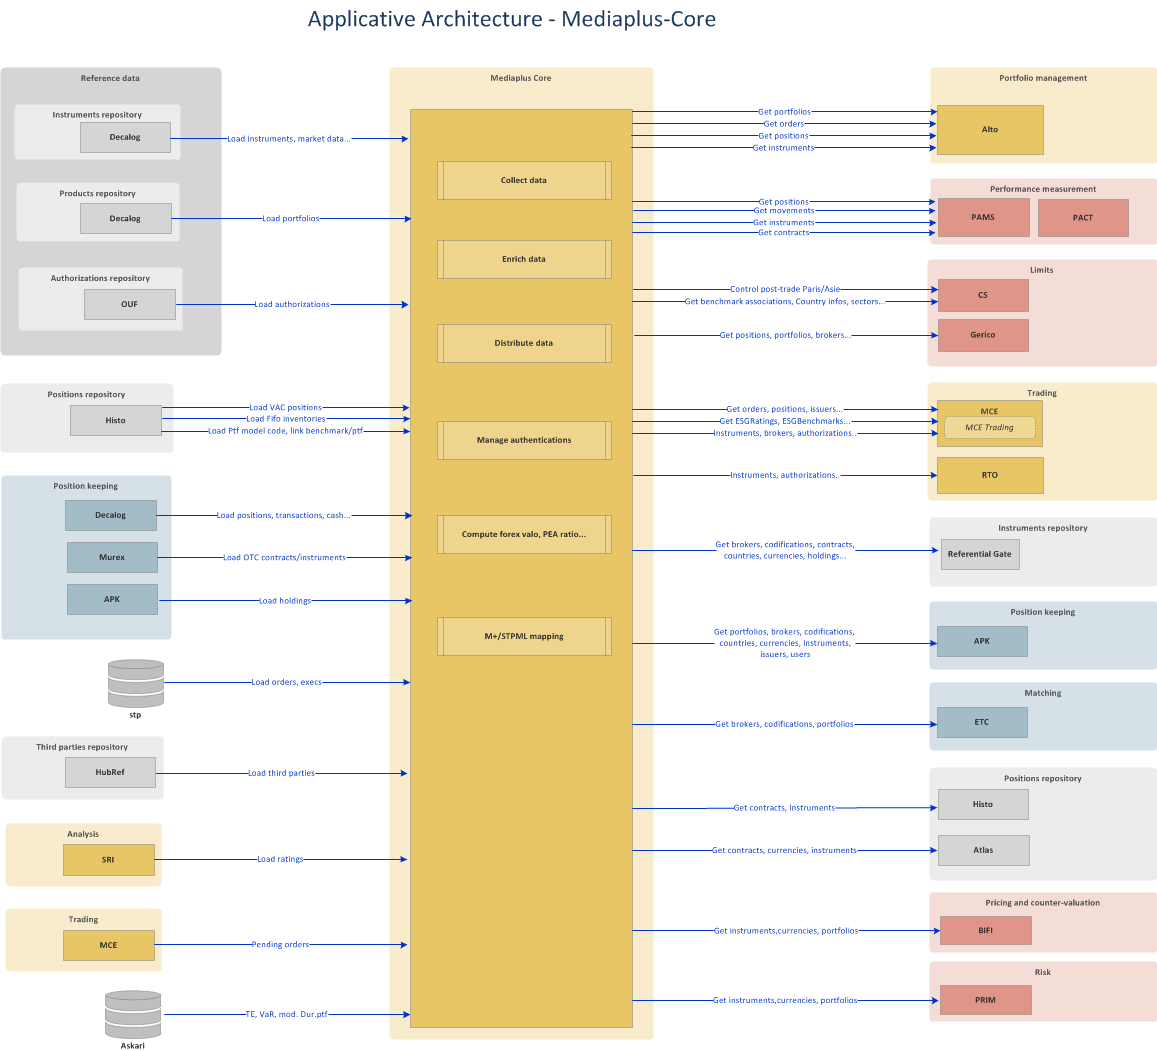
\includegraphics[width=\columnwidth]{img/Architecture Medco.png}
    \caption{Architecture applicative Medco}
    \label{fig:medcoArch}
\end{figure}
\par Sur la figure \ref{fig:medcoArch}, on retrouve a gauche les sources de données subdivisés en segments relatifs au type de donnée. Par exemple on retrouve les données référentiels extraite depuis DECALOG (pour les données instruments et produits), les données de position récupéré depuis DECALOG, une Base de donnée HISTO (Un autre type de base de données), ou l'application APK (Amundi Position Keeping) etc\dots
\par Comme le montre la figure \ref{fig:medcoArch}, Medco fait partie des plus importants serveurs centraux Amundi vu le nombre d'entrées et sorties. 


\section{Alto Investment Research}
\subsection{Cor}
\subsection{Masterdata SRI}
\subsection{Referential Widgets}

% Atlas
% BIFI
% DQC
% EWR
% FundLife
% Hubref
% Libra
% Life
% MDBM
% MDQC
% Medco
% OpenAml
% Refgt
% Refms
% rgp